\documentclass[10pt]{article}
\usepackage{tikz}
\usetikzlibrary{shapes.misc}
\usepackage[margin=0cm]{geometry}
\pagestyle{empty}
\tikzstyle{every node}=[cross out, draw, red]

\begin{document}

\vspace*{\fill}
\begin{center}
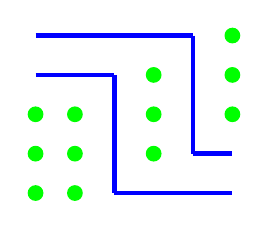
\begin{tikzpicture}[x=0.5cm, y=-0.5cm, ultra thick, blue]
% Walls
    \draw (0,0) -- (4,0);
    \draw (0,1) -- (2,1);
    \draw (4,3) -- (5,3);
    \draw (2,4) -- (5,4);
    \draw (2,1) -- (2,4);
    \draw (4,0) -- (4,3);
% Pillars
    \fill[green] (5,0) circle(0.2);
    \fill[green] (3,1) circle(0.2);
    \fill[green] (5,1) circle(0.2);
    \fill[green] (0,2) circle(0.2);
    \fill[green] (1,2) circle(0.2);
    \fill[green] (3,2) circle(0.2);
    \fill[green] (5,2) circle(0.2);
    \fill[green] (0,3) circle(0.2);
    \fill[green] (1,3) circle(0.2);
    \fill[green] (3,3) circle(0.2);
    \fill[green] (0,4) circle(0.2);
    \fill[green] (1,4) circle(0.2);
% Inner points in accessible cul-de-sacs
% Entry-exit paths without intersections
\end{tikzpicture}
\end{center}
\vspace*{\fill}

\end{document}
